%
% Simple LaTeX template for student theses
% - optimized for use with usual LaTeX editors
% - works without make file and changes to the directory structure
% - uses komascript for nicer layout (from European perspective)
% 
% v1, 2007 (Michael Brenner,MNM-Team,LRZ-M�nchen
% This version: v1.1, 2012 (Michael Brenner, MNM-Team, LRZ-M�nchen)
% adopted for FH L�beck by Andreas Hanemann


\documentclass[bibliography=totoc,listof=totoc,BCOR=5mm,DIV=12,oneside]{scrbook} 
% addition "`oneside"' for single-sided printing 
\usepackage[english]{babel}       
\usepackage{bibgerm} % deutsche Literaturverzeichnisse
\usepackage[latin1]{inputenc} % for German "`Umlaute"'
\usepackage{graphicx} % To insert figures  - for PDF-LaTeX: .pdf and .png (.jpg possible, but should be avoided)
\usepackage{url} % improve URL formatting (e.g. in the literature) 
\usepackage[onehalfspacing]{setspace} % for appropriate spacing
\usepackage{multirow}
\usepackage{multicol}
\usepackage{booktabs}
\usepackage{listings} %to display source code with \begin{1stlisting}... \end{1stlisting}
\usepackage{color}
\definecolor{lightestyellow}{rgb}{1,1,0.9}
\usepackage{hyperref} % takes care of links in pdf documents
% \usepackage{glossaries} glossary can be generated this way, not recommended for bachelor or master theses
% \makeglossaries
% \include{glossary} file glossary.tex could contain glossary terms, use of \newglossaryentry{} and \newacronym{} commands
%starting from here there are package which can be useful, turn on if needed; recommendations by Marco Trettner
% \usepackage{float} %for floats
% \usepackage{tabularx} %for tables
% \usepackage{ragged2e} %formatting of formulas or tables
% \usepackage{amsmath} %better math functions
% \usepackage{amssymb} %more math symbols
% \usepackage[decimalsymbol=comma]{siunitx}, um Werte mit ihren Einheiten sch�n darzustellen. Anstatt "I=5mA" schreibt man dann "I=\SI{5}{\milli\ampere}. Dann entsteht automatisch ein sch�ner kleiner Abstand zwischen dem Wert und der Einheit. Au�erdem wird die Einheit nicht kursiv geschrieben. Das geht nat�rlich nur in einer Mathe-Umgebung.
% \usepackage[nolist]{acronym} f�r Abk�rzungen. Dazu habe ich noch eine Datei eingef�gt mit "\input{acronym}", in der die Abk�rzungen in der Umgebung \begin{acronym}[Bash] durch z.B. \acro{IP}{Internet Protocol} aufgelistet werden. Im Dokument selbst gibt man dann nur \ac{IP} ein und das erste Vorkommen wird ausgeschrieben. Es gibt noch ein paar M�glichkeiten, die das Paket liefert. Z.B. wir durch \acp der Plural auch angezeigt, was manchmal sehr hilfreich ist. Das Argument [nolist] habe ich genommen, damit die Abk�rzungen nicht extra aufgelistet werden in einem Glossar.
% \usepackage{textcomp} f�r "TM" Symbole
% \usepackage[babel, german=quotes]{csquotes}; \usepackage[backend=biber, style=ieee]{biblatex} f�r Zitate mithilfe von Biblatex. Der Style "ieee" sorgt z.B. f�r die fortlaufende Nummerierung von Beginn an. Es gibt aber auch irgendwie 30 verschiedene Styles, die man einstellen kann.
% \usepackage{etoolbox}; \usepackage{hyperref} f�r URLs
% end of recommendations by Marco Trettner
\usepackage[backend=biber, style=alphabetic]{biblatex} %bibliography is generated via biber instead of Biblatex ; configure biber in development environment as needed
\addbibresource{./bib/thesis.bib}
\graphicspath{{./figures/}}
%
% der Befehl \hypenation versteht keine Sonderzeichen, also weder �
% noch "a noch \"a. W�rter die derartige Zeichen enthalten m�ssen
% direkt im Text getrennt werden, z.B. W�r\-ter
%
\hyphenation{Ma-nage-ment}
\hyphenation{Ma-nage-ment-agent}
\hyphenation{Ma-nage-ment-agent-en}
\hyphenation{Ma-nage-ment-ar-chi-tek-tur}
\hyphenation{Ma-nage-ment-ar-chi-tek-tu-ren}
\hyphenation{Ma-nage-ment-an-wen-dung}
\hyphenation{Ma-nage-ment-an-wen-dung-en}
\hyphenation{Ma-nage-ment-an-for-der-ung}
\hyphenation{Ma-nage-ment-funk-ti-on}
\hyphenation{Ma-nage-ment-funk-ti-onen}
\hyphenation{Ma-nage-ment-kon-zep-te}
\hyphenation{Ma-nage-ment-res-source}
\hyphenation{Ma-nage-ment-in-for-ma-ti-on}
\hyphenation{Ma-nage-ment-res-sour-cen}
\hyphenation{ma-nage-ment-re-le-vante}
\hyphenation{ma-nage-ment-sy-stem}
\hyphenation{ma-nage-ment-sy-steme}
\hyphenation{Ma-nage-ment-in-stru-men-tie-rung}
\hyphenation{Ma-nage-ment-platt-form}
\hyphenation{Sys-te-men}
\hyphenation{Sys-tem-um-ge-bun-gen}
\hyphenation{Sys-tem-ma-nage-ment}
\hyphenation{DHCP}
\hyphenation{Ma-nage-ment-diszi-plinen}
\hyphenation{System-management-architekturen}
\hyphenation{Verwendungs-nachweise}
\hyphenation{Video-einricht-ungen}
\hyphenation{Res-source}
\hyphenation{Res-sourcen}
\hyphenation{Grund-anwendung}
\hyphenation{Grund-anwendungen}
\hyphenation{Basis-anwendung}
\hyphenation{Core}
\hyphenation{Kom-mu-ni-ka-ti-on}
\hyphenation{De-sign-ent-schei-dung}
\hyphenation{Sprung-ad-res-sen}
\hyphenation{Klas-si-fi-ka-ti-on}
\hyphenation{Schreib-recht}
\hyphenation{Be-nut-zer-zer-ti-fi-kat}
\hyphenation{Bau-stein-ent-wi-ckler}
\hyphenation{ad-mi-ni-stra-ti-ve}
 % put words there it the separation does not work properly

% special commands by Marco Trettner; third one switched on by default
% \sisetup{exponent-product = \cdot, output-product = \cdot}
%Damit kriegt man die "X" bei der Darstellung von Exponentialzahlen zu einem Multiplikationszeichen gewandelt (4.5 x 10^3 wird zu 4.5 \cdot 10^-3)
%\lstdefinestyle{customC}{language=C, frame=lr, rulecolor=\color{blue!80!black}, keywordstyle=\bfseries\color{blue!80!black}, basicstyle=\footnotesize\ttfamily,}
%\lstdefinestyle{Console}{backgroundcolor=\color{white}, basicstyle=\scriptsize\color{black}\ttfamily}
%Das sind zwei Listing Styles, die ich f�r mich verwende, um C-Code oder um Konsolenausgaben anzuzeigen. Ist auch eine sch�ne Sache dieses Tool.
\apptocmd{\UrlBreaks}{\do\f\do\m}{}{}
\setcounter{biburllcpenalty}{9000}% Kleinbuchstaben
\setcounter{biburlucpenalty}{9000}% Gro�buchstaben
%Das ist ganz wichtig. Das durch Biblatex erzeugte Literaturverzeichnis kann Links enthalten, die mit \url erzeugt worden sind. Dabei kann es sein, dass die �ber den Rand hinaus gehen. Durch die beiden Befehle \setcounter wird einfach am Rand abgebrochen, sodass der Link noch funktioniert und die Optik beim Blockschreibsatz bleibt.

\begin{document}

% ---------------------------------------------------------------
\frontmatter % front pages and declaration
    \pagestyle{empty} % switch off page numbering
		%%%%%%%%%%%%%%%%%%%%%%%%%%%%%%%
% page as optional further cover page, optional

%\thispagestyle{empty}

%\begin{center}

%\vspace*{-2cm}

%\includegraphics[width=1.2\textwidth]{fhl_logo}

%\vspace*{5cm}

%{\Large \textbf{Bachelorarbeit}}\\ % oder Masterarbeit, Projektbericht, etc.

%\vspace{4.0cm}
%{\Huge \textbf{Anleitung zum Erstellen}}\\
%\vspace*{3mm}
%{\Huge \textbf{einer Abschlussarbeit}}\\
%\vspace*{3mm}
%{\Huge \textbf{}}\\
%\vspace{1.5cm}

%{\LARGE Andreas Hanemann} % Name des Autors

%\vspace{3cm}
%Entwurf vom \today % erleichtert den Betreuern die Zuordnung - f�r finale Version entfernen

%\end{center}

%\newpage

%%%%%%%%%%%%%%%%%%%%%%%%%%%%%%%
% second page

%\thispagestyle{empty}
%\cleardoublepage

%%%%%%%%%%%%%%%%%%%%%%%%%%%%%%%
% thrid page (mainly a copy of the first page)

\thispagestyle{empty}

\vspace*{-2cm}


\includegraphics[width=\textwidth]{thl_logo}

\vspace*{3cm}

\begin{flushleft}
	
	{\Large \textbf{Bachelor thesis}}\\ % oder Masterarbeit, Projektbericht, etc.
	
	\vspace{2.0cm}
	{\Huge \noindent\textbf{Instructions for Writing a}}\\
	\vspace*{3mm}
	{\Huge \noindent\textbf{Bachelor or Master Thesis}}\\
	\vspace*{3mm}
	{\Huge \textbf{}}\\
	
	\vspace{1.5cm}
	
	\begin{Large}
		\begin{tabbing}
			Submitted by: \hspace{.5cm} \=Max Mustermann\\
			\\
			\\
			Department: \>Electrical Engineering and Computer Science\\
			Degree program: \>Information Technology\\
			First examiner: \>Prof. Dr. Musterfrau\\
			\\
			Date handing in:  \>XXth month 20ZZ\\
			Date handing out: \>XXth month 20ZZ\\
		\end{tabbing}
		\vspace{5mm}
	\end{Large}
\end{flushleft}
\begin{flushright}
	\begin{Large}
		(Professor Dr. Andreas Hanemann)\\
		Head of Examination Board
	\end{Large}
\end{flushright}



 % title pages for FHL 
    \cleardoublepage
    \vspace*{2cm}

\begin{center}
    \textbf{Task description}
\end{center}

\vspace*{1cm}

\noindent International students face the challenge to write a thesis at the end of their studies. As many rules and examples of theses at the L�beck University of Applied Sciences are available in German exclusively they are not suited for the international students. Although many good guidelines are available online they do not cover the specialties of the L�beck University of Applied Sciences. Therefore, a special guideline is necessary. Besides very specific rules for this university some common mistakes are covered in this guideline.

\noindent The task for this work is:
\begin{enumerate}
\item Collection of the German guidelines and existing examples of successful thesis documents.
\item Analysis of the important rules and common mistakes of students when writing an English thesis.
\item	Creation of a comprehensive document serving as a template and a guideline for the students.
\item	Prepare a comprehensive Questions and Answers section.
\end{enumerate}

\noindent The deliveries are:
\begin{itemize}
\item A document that is well structured and serves as a guideline and template
\item A list of frequently asked questions + answers
\end{itemize}

 % abstract 
    \cleardoublepage
    
%

\newpage

\thispagestyle{empty}

\begin{large}


\includegraphics[width=\textwidth]{header_examinationboard}

\vspace*{2cm}

\noindent\textbf{Declaration of the Candidate}

\vspace*{1.5cm}

\noindent
I, the undersigned, hereby declare that the work contained in this thesis is my own original work, and has not previously in its entirety or in part been submitted at any university for a degree.
\vspace*{1cm}

\noindent Only the sources cited in the document have been used in this draft. Parts that are direct quotes or paraphrases are identified as such.
\vspace*{1cm}

\noindent I agree that my work is published, in particular that the work is presented to third parties 
for inspection or copies of the work can be passed on to third parties.
\vspace{2cm}

\noindent
L�beck, Month XXth 20ZZ

\vspace{3cm}

\hspace*{7cm}%
\dotfill\\
\hspace*{10cm}%
\textit{(signature)}

\end{large}
 % declaration (own work)
    \cleardoublepage
    \vspace*{2cm}

\begin{center}
    \textbf{Zusammenfassung der Arbeit / Abstract of Thesis}
\end{center}

\vspace*{1cm}

\begin{table}[htb]
  \centering
  \begin{tabular}{lp{10cm}}
    \toprule
    \textbf{Fachbereich:} & \multirow{2}{*}{Electrical Engineering and Computer Science} \\
		\textbf{Department:} & \\
    \midrule
		\textbf{Studiengang:} & \multirow{2}{*}{Information Technology} \\
		\textbf{University course:} & \\
		\midrule
		\textbf{Thema:} & \multirow{2}{*}{Instructions on Writing a Thesis} \\
		\textbf{Subject:} & \\
		\midrule
		\multirow{2}{4cm}{\textbf{Zusammenfassung:} \textbf{Abstract:}} & The following work is a short guide for writing a thesis. It is intended for final-year students of international programs at L�beck University of Applied Sciences. This document serves both as example and as a thesis template following the formal requirements of the final thesis, such as the layout, font-style, structure, etc. This template was created with LaTeX. Students can use this template as a reference guide or replace all text in the front part of this template with their own information and customize it to suit their needs. This will save lots of efforts for the students when formatting the thesis. \\
		\midrule
		\textbf{Verfasser:} & \multirow{2}{*}{FirstName Surname} \\
		\textbf{Author:} & \\
		\midrule
		\textbf{Betreuender Professor:} & \multirow{2}{*}{Prof. Dr. FirstName Surname} \\
		\textbf{Attending professor:} & \\
		\midrule
		\textbf{WS / SS:} & SS 20XX \\
		\bottomrule
  \end{tabular}
\end{table}

 % optional
    \tableofcontents % table of contents
		\addtocontents{toc}{\protect\thispagestyle{empty}}

% ---------------------------------------------------------------
\mainmatter % main part of the work
    \pagestyle{plain} % switch on page numbering
    \chapter{Introduction} \label{chap_introduction}

\section{Motivation}

The final thesis is an integral part of international students' study at L�beck University of Applied Sciences (THL). Although final-year students have already spent several years studying in English before working on their theses, many of them do not know how to write such a specific-purposed document. Admittedly, there are many thesis guidelines and related literature available (e.g. \cite{les06}), but each university has its own rules and requirements for writing a thesis. Therefore, it is highly desirable that a thesis guideline/template be provided specially for the international students at THL.

The authors of this document in chronological order are Horst Hellbr�ck, Zhi Haolin, Aida Bahta, Ren Zhong and Andreas Hanemann. Horst Hellbr�ck has started the document and the structure in 2009 with Zhi Haolin providing most of the texts in the first version. Ren Zhong has rewritten and rephrased most of the texts and extended the documentation in 2012 resulting in this comprehensive guideline. Further additions have been made by Andreas Hanemann in early 2013 using input from Aida Bahta and further THL instruction documents. Andreas Hanemann has also converted the Word template into this LaTeX template.

Important: This document is not a legal basis. Refer to the examination regulations. The instructions of the supervisor are authoritative for the student's thesis.

\section{Goal}

This document is intended to assist the final-year students in the international study programs at THL to write their theses. The goal of the document is twofold. On one hand, it serves as a guideline for the students looking for practical help, including structure, language, writing strategies, format, etc. On the other hand, this document is also a template of a thesis created with LaTeX (more precisely MikTeX in combination with TeXstudio under Microsoft Windows; Biber is used instead of Bibtex). It strictly follows the formatting requirements for a thesis at THL. Students are encouraged to replace the text with their own content and use this template as a starting point of their theses.

\section{Organization}

The rest of the document is structured as follows. Chapter \ref{chap_process} explains the procedure for writing a thesis at THL. It comprises the colloquium as well. Chapter \ref{chap_structure} explains the typical structure for a thesis and provides a typical example. Chapter \ref{chap_writing} discusses the use of language in a thesis and specifies the formatting requirements. Chapter \ref{chap_summary} summarizes the work, and suggests future work that could be done to improve this document. In the Appendix a list of frequently asked questions covers many questions often asked by students.

\endinput

    \chapter{Work on the Thesis} \label{chap_process}

This chapter explains the procedure for writing a thesis at THL. 

\section{Thesis registration form}

Approx. three weeks in advance of the start it is necessary to begin the process to check the fulfillment of requirements for writing a thesis at the secretariat. The student can either fill out a form at the secretariat directly or can ask via e-mail to ei@th-luebeck.de to perform the checks. This does not mean that the student is immediately registered for the thesis, it is just a check of requirements. If all requirements are fulfilled with respect to the examination regulations, the first advisor will get a notification (with CC to the student). The first advisor then provides the title, official start date, and may also provide a task description. This official start date determines the final thesis hand-in date three months later (six months in case of master thesis).

First advisor of a thesis can in general be any member of the faculty as long as the scientific area of this person matches to the topic of the thesis. For some members of the faculty who are not professors it is necessary that their role as first advisor is confirmed by the examination board.

Remark for Chinese students: Since all Chinese students start their theses on the same day, a special procedure applies. Please note the remarks on this in the lecture of Ms. Hanesova.

\section{Specification of a thesis subject}

Several situations are possible for finding a thesis topic.

\subsection{Given topic}

It is possible that the first advisor already has a clear idea about a subject. She or he may already provide a title and also a description of the task. Nevertheless, a discussion of the subject and the tasks should take place between student and first advisor. It is possible to change or improve the task description as a consequence of this discussion. The student should verify together with the first advisor that those aspects as discussed in Section \ref{sec_newtopic} have been taken into account. 

Remark: This is the typical situation for Chinese students doing their work inside of THL.

\subsection{Joint specification of a topic} \label{sec_newtopic}

For theses where the student has a proposal for a subject (which is often the case for theses in cooperation with companies) it is necessary to jointly specify a task description. The proposal for the topic and task description draft should be provided in a written manner by the student. One or two pages are sufficient for that. The (potential) first advisor should get the possibility to judge from the description whether the topic is suited for a thesis. The description should comprise a draft for an outline. 

The following aspects are relevant for the task description:
\begin{itemize}
\item The choice of the subject needs to reflect a suitable challenge and effort. On the one hand, this means that the topic for a bachelor thesis has to be appropriate to address it within three months. These three months have to be sufficient even if unexpected difficulties arise (e.g. hard to find programming errors; unclear requirements which become apparent later). On the other hand, the topic needs to require knowledge which has been gained throughout the studies. Very often a combination of theoretical considerations combined with a (prototypical) practical implementation is chosen. A task description which means just an implementation of given concepts would be regarded as not sufficiently demanding.  
\item The task description together with the outline needs to address the following questions: 
  \begin{itemize}
  \item What is the main problem? It should be tried to answer this question precisely in one or two sentences.
  \item Why is it important to find a solution for the problem?
  \item Why are existing solutions regarded as insufficient?
  \item How is the way to address the problem? 
  \item How can it be checked (later on) whether the developed solution actually solves the problem? This is typically done by a catalog of criteria which needs to be developed first.
  \end{itemize}
\item The thesis has to match with scientific standards also in cases where the thesis is done in collaboration with an external company. The steps which are taken in the course of the thesis need to have technical reasons. An argumentation that a certain way to address a problem is desired by senior employees is not allowed. The thesis needs to be approached in an objective manner and not with respect to the company's views. This is also necessary for the written thesis where it is unacceptable to repeat advertisement messages of the company (e.g. ``company X the worldwide leader in manufacturing of product Y ...''). 
\item The student should consider her or his own professional future in the cooperation with the company. For instance, it should be taken into account whether work similar to the one conducted throughout the thesis is also interesting for the student on the long run. The choice of the topic will be subject of hiring talks in the future and can be helpful to show skills in an area that matches to the offered job.
\item The task description and title of the thesis need to be considered carefully so that it is possible to get a clear idea of the topic, but also to show that it is a challenging topic. It is important to note that the title is chosen at the beginning and cannot be changed afterwards.
\end{itemize}

The official task description is derived from the proposal as Word or simple text file in collaboration with the first advisor.

For many theses there is a preparation of the work in front of the official registration of the thesis. This is a common procedure in particular in the collaboration with companies.

Remark for Chinese students: Due to the strict time line a preparation of work is only possible in February and March in front of the official registration in the second half of March.

\section{Registration form back to secretariat (via first advisor)}

Based on the task description which is provided on the form the secretariat derives the official task description. The official source of the topic and task description is the examination board represented by its head. The student does not write anything on the form. A request to fetch the official task description is sometimes provided by paper mail.

\section{Thesis duration}

The thesis has to be finished until a predefined date and needs to be completed with respect to the required formalities. The duration of a bachelor thesis is three months. A master thesis takes six months.

\section{Advice}

There are differences between the advice for internal and external theses.

\subsection{Advice for an internal thesis}

For the advice on internal theses it is common to agree on weekly or biweekly meetings. It is sufficient in many cases if conducted and future work is discussed orally.

\subsection{Advice for an external thesis}

For an external thesis in a company short written reports which are sent via e-mail are better suited. They may be sent for a time interval of three weeks for example. For those reports the following outline is suitable: Student name, thesis title, report date, report interval, status (e.g.~implementation, measurements, calculations, or simulation), results (same category, but concrete work, e.g. finished prototype platform), documentation (specific information, e.g.~finished related work chapter), plan for the next time interval (specific information like: measurement preparation in the next week, conducting of measurements in the following week, finish measurement report in the third week). Those short reports are helpful for planning and for the early detection of timing issues.

During the work at an external company the first advisor will visit the students as needed. The agreement on the date of the visit is usually done via e-mail. 

\subsection{Intermediate versions of the thesis}

The student sends intermediate versions of the thesis to the advisor. This holds both for internal and external theses. The student should use version numbers in an obvious way and should mark for the advisor which parts of thesis are new or have been revised significantly. This is eases the correction work for the advisor. 

\section{Second advisor}

Approx.~four weeks before the end of the work on the thesis the student should get in contact with a second advisor. The second advisor should be familiar with the scientific area to which the subject of the thesis is related. The first advisor can be asked for help to recommend a second advisor.

Important: The student has to take care of the coordination of dates.

\section{Deadline and submission}

The submission of the demanded \textbf{two hard copies} can be done by personal delivery to the secretariat or be done via paper mail (address: Technische Hochschule L�beck, Fachbereich Elektrotechnik und Informatik, Pr�fungsausschuss, M�nkhofer Weg 239, 23562 L�beck, Germany). In the second case, the postmark stamp fixes the submission date. In addition to the written thesis the thesis itself and further material (program code, etc) has to be put on a CD and has to be attached to each hard copy (inside of the back cover). One of the hard copies will be archived later. The second one is checked by the first advisor and will remain in her or his office. 

The \textbf{deadline} has to be met in any case since the thesis is regarded as \textbf{failed} otherwise. An exception is only possible in case of third party mistakes (e.g.~if the external company has not delivered important documents as promised) or in case of illness. In these situations a request for a prolongation of the thesis duration has to be posed in front of the expiry of the submission date. A deadline extension due to an inaccurate time organization of the student is not possible. The topic of the thesis may be returned once within the first one-third of the thesis duration. This has to be stated in a written manner towards the examination board. If the thesis is regarded as ``failed'' at the end, a second attempt (but no third attempt) is possible (the request for doing a second attempt has to be posed within the next two semesters). 

The submitted thesis copies must be printed and bound to archives. The binding can be done in the print office in building 36, but also in town. Students should not have the thesis bound until the supervisor has approved the final draft, including all extra pages both preceding and following the main text. There are two types of binding available as illustrated in Figure \ref{fig:bindings}. Both simple binding and hard binding are allowed. However, it is a good idea to ask the supervisor for her or his choice. The student should make sure that all pages are there and that they have the right order.

%Figure from PNG-File - take care that the figure has a sufficient resolution (so that a scaling >300dpi can be used in the printout) 
\begin{figure}[htb]
  \centering
  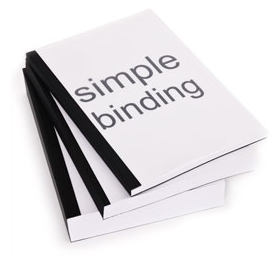
\includegraphics[width=.4\textwidth]{simple_binding} % PNG-File
	
\includegraphics[width=.4\textwidth]{hardcover}\\ % PNG-File
  \caption{Simple binding (left) and hard cover (right) \cite{coll13}}\label{fig:bindings}
\end{figure}

Sometimes it is useful to make more hard copies, e.g.~for employees from companies where the thesis work has been done.

Remark for Chinese students: Please consider that the same deadline holds for the other students as well. Therefore, queues are possible if everyone wants to print the thesis on the same day.

\section{Finding an oral examination date}

The student should agree with the advisors on the date, time and place of the oral examination (called ``colloquium'') well in advance. Dates outside of the lecture weeks can be hard to arrange. The student should ask the advisor about her or his ideas on the course of the colloquium (exact duration of the presentation, use of media, short demonstration possible).

\section{Colloquium}

The student prepares a slide set for the colloquium which is designed to take 25 minutes to be presented (deviations are possible in particular for online degree programs, check with first advisor). It is estimated that it takes two or three minutes to present a single slide so that approx.~10 slides should be used. Spelling mistakes on the slides should be avoided. The presentation may include the use of a blackboard, the showing of physical prototypes or a short demonstration.

The focus of the slides should be the work that the student has done. This means that it is inappropriate to spend too much time on explaining the background or discuss related work. Often the student can use a similar outline as the one used in the written thesis. An important difference is that the presentation should not strive for completeness, but can select specific examples. A file with advice on the colloquium slides can be found in the folder about the presentation.

The colloquium itself takes place in a seminar room or a small lecture room. During the time of the presentation the public can participate, but the public is excluded when the advisors pose their questions. It is a pity that the colloquium often takes place without additional listeners which is inappropriate in relation to the effort that is invested into many theses. The student should check the availability of the technical equipment in advance. She or he should be in the room on time to cope with (frequent) difficulties, e.g. that the beamer does not want to cooperate with the notebook, and to resolve them before the start of the colloquium.

At the end of the colloquium the presentation should be delivered to the first advisor.
 
\endinput 
	\chapter{Structure} \label{chap_structure}

A thesis must be a coherent document of a research project, not a collection of loosely connected pages. This chapter walks through the typical structure of a thesis from cover to cover, and discusses the aim and content of each part. Sections \ref{sec_coverpage} through \ref{sec_declaration} describe the mandatory pages that must be included in each thesis.

\section{Cover page} \label{sec_coverpage}

The cover page is officially provided by THL and signed by the supervisor and the board of examinations, as can be seen at the first page of this document and in Figure \ref{fig:coverpage}. Students will receive an original version and a black-white copy of the official cover page, each of which serves as the cover of the two thesis copies.

\begin{figure}[htb]
  \centering
  
\includegraphics[scale=.8]{titlepage_small}\\
  \caption{Example of a page 1 - Cover page}\label{fig:coverpage}
\end{figure}

\section{Task description}

The task description covers some background information about the thesis, lists the major steps during the work, and specifies the deliverables of the thesis. It can be seen as a contract between the student and the supervisor or the company and is the basis for grading. Therefore, students should make sure the listed tasks are reasonable to be finished within the time constraints. Figure \ref{fig:task} shows an example of this page.

\begin{figure}[htb]
  \centering
  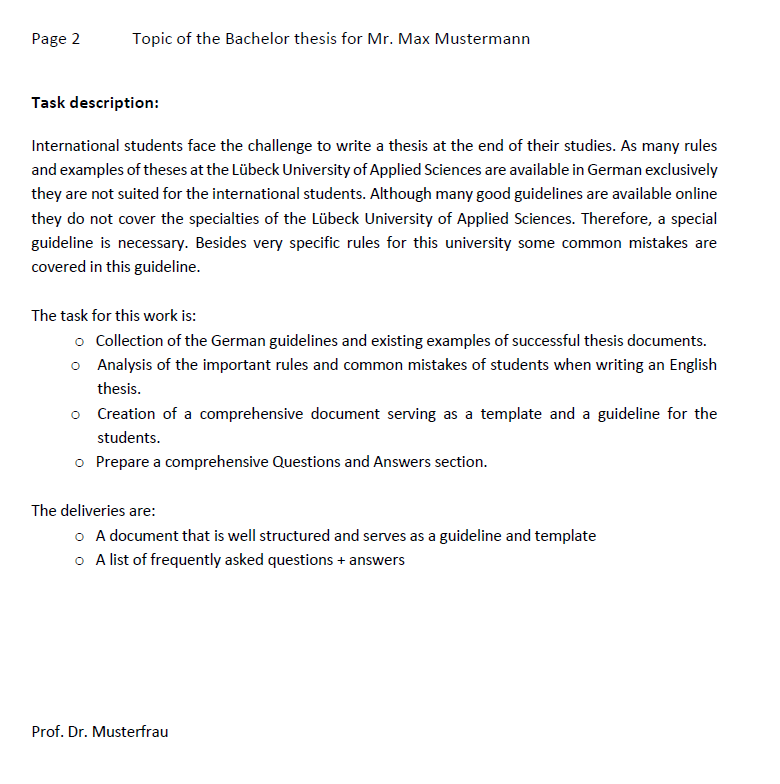
\includegraphics[scale=.8]{thesistask_small}\\ 
  \caption{Example of a page 2 - Task description}\label{fig:task}
\end{figure}

\section{Declaration} \label{sec_declaration}

Students are required to sign the declaration of the thesis provided by THL (see Figure \ref{fig:declaration}), which includes \cite{kun08}:
\begin{itemize}
\item The fact that she or he writes the work independently without outside help.
\item The fact that she or he has used only the cited sources.
\item The fact that she or he agrees with a publication of the work.
\end{itemize}

The first two items are mandatory while the last one is optional. Pay attention that some students working in companies are required to sign a Non-Disclosure Agreement (NDA) with the companies, and some companies do not agree to publish the thesis work. In this case, the last paragraph must be removed from the declaration.

%Figure from pdf file - preferred option since it allows to include true vector graphics 
\begin{figure}[htb]
  \centering
  
\includegraphics[scale=.4]{thesis_statement}\\ % PDF-File
  \caption{Declaration form}\label{fig:declaration}
\end{figure}

\section{Abstract}

The abstract is one page maximum, including information from the cover sheet plus the abstract of the work. By default the secretariat will hand out a form that the students can fill in. Many students, however, have developed their own page for this purpose. 

The abstract is one of the most important parts of a thesis, because it leaves the very \textit{first impression} of the following text. It has to be \textit{self-contained}, which means it can be understood separately from the thesis itself. 

\section{Table of contents}

A table of contents is a list of all chapters and sections with page numbers. It enables the readers to easily find information they are looking for. A LaTeX command automatically generates the table of contents.

The titles of chapters and sections should have a good naming so that the reader can easily imagine what the content is about. This is important if the thesis is briefly read by someone (e.g.~from a company that considers to hire the student) in the future who wants to get an impression whether the work has been carried out in a good way.

The work should be provided as a pdf file later. It is nice if the table on contents is linked with the sections so that a click on a section title in the table of contents leads to a jump into the section. A similar functionality should also be provided for other links (e.g.~to the bibliography). This functionality is already contained in this LaTeX template, but should be conserved when converting it into pdf.

\section{Chapter 1: Introduction}

The purpose of the introduction is to stimulate the readers' interest and guide the reader into the subject. Before writing a good introduction usually the author needs to know the body of the thesis, so it is suggested to write the introduction after completing the rest of the thesis.

An introduction typically contains 3 basic parts \cite{les06}:
\begin{itemize}
\item Background or motivation of the thesis
\item Goal of the thesis
\item Organization of the following chapters 
\end{itemize}

The first part briefly states what the problem is and why it is desired to address this problem in the thesis. The second part presents the goal to be achieved in this thesis, i.e. solution to this problem. It is not a good idea to transfer the text from the task description into this chapter. Students are expected to explain the problem and the goal in their own words. Finally,  a preview of the rest of the document should be provided chapter by chapter to tell the reader what can be expected.

The benefit of a preview is that the reader will be able to scan the thesis at first and have a good sense of what will be covered in each chapter. This allows the reader to select individual chapters if she or he wants to skip parts of the document. To make the thesis as readable as possible, it is suggested to use this strategy throughout the thesis by writing an introductory paragraph at the beginning of each chapter (or even some sections if necessary). See the beginning of the next section for a simple example.
  
\section{Chapter 2 to N-1: Main body} 

The body is the major component of the thesis. It describes how the author accomplished the task step by step and how she or he achieved the results. There is no fixed structure of the main body, as it may vary according to the task description, but Section \ref{sec_examplestructure} describes a common way of organizing the chapters. Section \ref{sec_pitfall} introduces a common pitfall in writing the main body the thesis.

\subsection{Example organization} \label{sec_examplestructure}

In computer science topics there is often a task description which foresees the development of a theoretical concept combined with a prototypical implementation. The following outline can be used in this case.

In the second chapter the problem is analyzed in depth by using one or several scenarios. At the end of the chapter there is a list of requirements which have to be fulfilled to provide a solution to the problem. The requirements do not have to be pure technical requirements, but may include license issues and economic constraints (e.g.~low investment costs).

In the third chapter literature and related work (in standardization documents, research papers, and existing systems) is examined whether there is already a solution to the problem. This should not be the case because the work would otherwise already be finished in this chapter. At the end of this chapter a table is provided which shows the examination results and details which requirements are fulfilled by each existing approach. All related work has to cover some smaller or bigger part of the requirements. Otherwise, they cannot be regarded as related work, but it is necessary to point out their deficits with respect to the problem.

In chapter four a theoretical approach to the problem is drafted. Often a basic idea for the solution of the problem is presented at the beginning which is elaborated afterwards. At the end of the chapter the developed solution is compared to the requirements to verify whether all of them are fulfilled. This should be the case for the mandatory requirements. Some optional requirements may not or partially be fulfilled.

In the fifth chapter a practical implementation of the theoretical concept is presented. Technical information on the implementation is given, e.g.~used programming languages, development tools, hardware, etc. This chapter demonstrates that the theoretical solution works in reality.

It is important to note that the structure of the thesis does not match to the actual way how the thesis subject has been addressed. For many chapters material is collected at the beginning and is drafted as bullet point lists. Towards the end of the thesis time it is converted into text. In addition, it has to be checked before the start of the thesis that there is no perfect solution available for the problem which can be applied easily.

The first advisor for the thesis can give recommendations on how to structure the thesis. A discussion on this should happen relatively early after the start of the thesis.

\subsection{A common pitfall} \label{sec_pitfall}

While writing a thesis, the student has only limited time, energy and number of pages to describe the work which has been accomplished. Hence, some parts need to be elaborated while others just briefly mentioned. In general, it depends on the significance of the particular part of the work. 

However, one common pitfall is that some students devote too many pages describing the detailed software implementation and put many blocks of code in their thesis. Even if the majority of the thesis is about software implementation, one should not describe too many details of the source code. What should be elaborated and emphasized is the class interfaces, program framework, design considerations and implementation trade-offs behind the trivial details. As will be mentioned in Section \ref{sec_CD}, an enclosed CD will provide the entire source code for reference. Consequently, include source code only when it helps to clarify significant issues.

\section{Chapter n: Conclusion and outlook}

The final chapter comprises the major results of the thesis and the outlook. It summarizes the achievement and the results of the work in technical terms. At this point it can be assumed that the previous chapters of the thesis are known to the reader (in contrast to the summary at the beginning). Nevertheless, it should be taken into account that there are quick readers who have skipped several chapters and just want to have an impression of the major findings of the work.

The outlook proposes future possible extensions or challenges of this work. Optional requirements which have not or only partially been fulfilled may give a hint for this.


\section{Acknowledgements}

The author is free to acknowledge the supervisor(s) and anyone who helped the author: 
\begin{itemize}
\item Technically (including materials, supplies)
\item Intellectually (assistance, advice)
\item Financially (for example, departmental support, travel grants, parents)
\end{itemize}

\section{Appendices}

Appendices can include the list of figures, tables or listings and other materials which are either too long to be inserted into the main chapters of the thesis, or which are interesting, but not essential to understand the main text \cite{les06}.

\section{Bibliography or references}

In this section, the student should provide a list of referenced literature in alphabetical order or in the order that the references appear in the main text. Each entry in the bibliography has to be mentioned at least once in the main text. For the formatting of bibliography, please refer to Section \ref{sec_citations}.

\section{Enclosed CD} \label{sec_CD}

If software implementation is an important part of the thesis, it is recommended that a CD containing the source code be enclosed on the back cover of the thesis.

\endinput 
    \chapter{Advise on writing the thesis} \label{chap_writing}

The thesis is an own scientific work of the student. It will be read in any case by the first and second advisor, but it should be written in a way that it is understandable to anyone from the corresponding scientific area without the need to read additional literature. This holds in particular for employees of companies where the work has been carried out (in case of external theses).

\section{Number of pages}

It is not possible to give a general recommendation for the reasonable length of a thesis. This depends on the subject. For instance, a subject which includes a detailed comparison of related work may require more pages than a subject with a focus on the practical implementation. Table \ref{tab:pages} contains some suggestions for different kinds of theses.

% Tables can be put in a figure environment - the use of a table environment is in particular usefulif many tables are included
\begin{table}[htb]
  \centering
  \begin{tabular}{|l|p{3cm}p{3cm}p{3cm}|}
    \hline
    \textbf{Type of work} & \textbf{Minimum} & \textbf{Average} & \textbf{Maximum}\\ \hline
    Project report & 10 pages  + appendix (+ CD) & 15 pages + appendix (+ CD) & 30 pages  + appendix (+ CD)\\ \hline
    Bachelor thesis & 30 pages + appendix + CD & 45 pages + appendix + CD & 100 pages + appendix + CD\\ \hline
		Master thesis & 60 pages + appendix + CD & 75 pages + appendix + CD & 130 pages + appendix + CD \\
    \hline
  \end{tabular}
  \caption{Suggestions for the number of pages}\label{tab:pages}
\end{table}

Please note that the number of pages does not have an implication whether the thesis is good or bad (Einstein's PhD thesis had 17 pages). As discussed in the writing style section it is better to be precise and short rather than to describe something with many words.

\section{Writing style}

A thesis document is comparable to a research report or scientific book, like Tanenbaum's ``Computer Networks''. Scientific writing has to be a formal document - much more formal than many articles in the Internet. Colloquial and informal writing is undesirable.

Formal and informal English differ in word choice, word usage, and grammatical structures. Informal writing might utilize the words ``kid'', ``how come'' and ``quote'' as a noun. A formal writer might prefer ``child'', ``why'' and ``quotation'' \cite{sch96}. 

Non-native speakers should note that the word-by-word translations from another language like Chinese or German does not work in writing a thesis, so students are suggested to always use an English book as a reference for language.

Three keywords for scientific writing are \textit{clarity}, \textit{precision} and \textit{brevity}. They can serve as the watchwords to ensure a thesis is readable, persuasive and concise. Pages 18-26 in \cite{cha02} provide some very useful hints on understanding the three words and discusses some other issues on the use of language in thesis writing.

An important stylistic choice in scientific writing is between active voice and passive voice. One way to express what was done is to e.g.~say ``I performed frequency measurements''. In this way it becomes obvious what was done by the author. However, this kind of writing is uncommon in scientific work and should be used only when there would be uncertainties about who contributed which pieces of work. A better alternative writing to make this obvious is use a sentence similar to ``Frequency measurements were conducted by the author''. In most situations a passive form like ``Frequency measurements were conducted'' is the best option. 

In a scientific thesis it is very unusual to address the reader directly as ``you''. Thus, one should change sentences like ``This chapter tells you the reason why ...'' to ``This chapter gives reasons why ...''.

\section{Active verbs}

Using precise, active verbs can make the thesis more concise, precise and persuasive. For example, instead of saying ``This work is a generalization of Smith's earlier algorithm.'', it is better to write ``This work generalizes Smith's earlier algorithm.'' \cite{hew03}.

Some frequently used active verbs include: present, summarize, illustrate, clarify, reveal, introduce, indicate, propose, specify...

For more useful hints and a list of active verbs, please refer to \cite{hew03}.

\section{Transitional words and phrases}

Transitional words and phrases provide the glue that holds ideas together in writing. They help the reader to understand the relationships between ideas, and can be used to connect sentences, paragraphs, or even entire sections \cite{har11}.

The following paragraph is an example on how transitional expressions establish relationships between ideas and connect sentences to form a logical chain. In order to notice the difference read the paragraph with and without the words in \textit{italics}.

``\textit{Unlike} some common protocols \textit{such as} UDP, the original CCN protocol does not have any fixed-length fields in the messages. \textit{Instead}, the message formats are defined by XML schemas \textit{and} each field can be of arbitrary length ...

Such protocol design, \textit{however}, is not applicable to wireless sensor networks, which generally have very limited communication bandwidth. \textit{In particular}, the MAC layer frame size on our platform is merely 127 bytes ...''

Some more suggestions and a well-organized list of transitional words and phrases can be found in \cite{har11} and \cite{poss} (both online).

\section{Tenses}

Usually the thesis should be written in present tense. Sometimes it may be necessary to describe steps which have led to a current result. In this case it can be useful to use the past tense to explain the steps. It is important to use the tenses in a consistent manner.

\section{Formatting requirements}

The following layout settings are suggested for a thesis.
\begin{description}
\item[Paper:] A4
\item[Font:] Times New Roman 12pt or Arial 11pt; the font sizes should be at least 11 pt; no fancy fonts should be used
\item[Justification:] Use justification; avoid empty spaces by appropriate word separations
\item[Margins:] All around 2.5 cm (0.98 inches)
\item[Spacing:] one half spacing; is achieved by using the \textit{setspace} package 
\item[Page use:] single sided print for the two final printouts; the option \textit{oneside} in \textit{documentclass} is activated in this template 
\item[Tables:] For the table of contents, table of figures, etc there is no need to write them by hand. Use LaTeX commands to generate them automatically.
\end{description}

\section{Emphasis}

In scientific writing, there are several ways to highlight or emphasize some words or phrases within a paragraph, including \textbf{boldface}, \textit{italics}, \underline{underlining} and CAPITALIZATION. Generally speaking, boldface and italics are recommended while underling and capitalization should be avoided. However, even boldface and italics should be used \textit{sparingly} (especially boldface), because too many highlights will just do the opposite.

A student can use either boldface or italics or both in her or his writing, but the usage should be \textit{consistent} throughout the entire thesis. There is a subtle difference between boldface and italics. Within a large body of text, a word in \textit{italics} does not stand out much. Instead, it signifies a context difference only \textit{while} the text is being read. It is useful for highlighting the introduction of new terms. In contrast, a word in \textbf{boldface} can easily attract human eyeball and is therefore recommended for keywords that the readers might be looking for \cite{wik13a}.


\section{Citations} \label{sec_citations}

It is necessary to cite if foreign work has been included into the thesis. A reference has to be added which points to the bibliography and the bibliography has to contain enough information to find the sources. There are multiple standards on the format of citations. For scientific writing, the IEEE citation style is usually recommended. The detailed IEEE citation standard can be found online in \cite{ieeecitation09}. The BibTeX file belonging to this template contains examples for references to different sources.

The use of footnotes is possible, but is not recommended because it leads to a replication of information if the same source is cited multiple times (there may be a pointer to an earlier footnote to avoid this, but this solution is inconvenient for the reader). In addition, the use of footnotes disrupts the reader from the main text and is rather uncommon in electrical engineering or computer science documents in contrast to other scientific areas. 

Citations which use the wording of the foreign text need to be indicated with quotation marks. In electrical engineering and computer science word-by-word quotes are not useful in many cases and should be avoided. If they are used, they should be as brief as possible. It is preferable to explain something by using one's own words (it is of course still necessary to point to the source). One exception is the definition of important terms since an explanation using own terms may easily lead to a loss of precision. In this case the source needs to be provided with a detailed reference, e.g. indicating the page in a book.
 
When referencing Internet pages it needs to be taken into account that these may be changed over time. There should be a remark when they have been accessed for the last time. They should be downloaded (if possible) to make sure that the content is preserved.

\section{Figures and tables}

Figures and tables are always a good complement to the written text. They can visualize some complicated concepts or ideas, and help the readers understand the text better. Especially for those theses involving programming, a \textit{class diagram} can easily clarify the design of a program.

Similar to the use of boldface and italics, figures and tables should also be used \textit{sparingly} and \textit{selectively}. A common pitfall is to include too many screenshots in the thesis. Remember a thesis is basically a formal record of the author's original research, not a software tutorial or a user manual. Each figure has to provide an added value for the reader. This does not hold for company logos or startup screens.

Each figure or table should be labeled with a caption briefly stating its content. If the figure or table is taken from elsewhere, a reference has to be included in the caption as well.

Figures and tables are illustrations that complement the text. These illustrations can \textit{never} substitute text. Consequently, figures and tables need to be described and referenced in the text accordingly. A common pitfall is that students expect the reader to ``read'' the figures. A figure which is not referenced will may be considered by the reader, because she or he does not know when to look at the figure.

\section{Program code}

In computer-related books and articles, a piece of code is formally referred to as a listing or program listing. Similarly, program listings should also be used very sparingly, as all the source code will be available in the enclosed CD. Like figures and tables listings can only be used as a complement to the written text. Sometimes it is useful to explain something with a pseudocode rather than to provide all details of the actual code. 

Although there is no universal format for a listing, some basic rules should be followed. First, a listing should always be labeled, just like a figure or a table. Second, the font for the code should be mono-spaced (e.g. Courier New, etc.). Figure \ref{fig:examplecode} is a simple example of a listing (the format is not required but recommended).

\begin{figure}[htb]
  \centering
  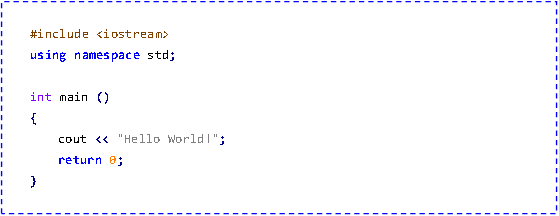
\includegraphics[width=.7\textwidth]{examplecode}
  \caption{Program listing example}\label{fig:examplecode}
\end{figure}

If a thesis contains only very few program listings, they might also be labeled as figures and included in the List of Figures. Otherwise, it is suggested to provide a List of Listings.

\lstset{emph={int,for},emphstyle=\normalfont \ttfamily\color{red},
backgroundcolor=\color{lightestyellow},
stringstyle=\normalfont \ttfamily,
basicstyle=\normalfont \ttfamily,
numbers=left}
\begin{lstlisting}[frame=trb,captionpos=b,caption=Display of program code using 1stlisting,label=lst:examplecode]
int $i;
for($i = 0; $i < 10; $i++) {
echo $i;
}
\end{lstlisting} 

Alternatively the program code can be shown by using a special LaTeX package named listings. The listing \ref{lst:examplecode} serves as an example.

If the thesis involves programming work, it is recommended to use code versioning software. In the material folder a Subversion tutorial is provided for this.

\section{Acronyms and terms}

The use of acronyms is common in scientific writing since it keeps the brevity of the text. However, when using an acronym for the first time, the phrase should be spelled out and followed by the acronym in parentheses (not in a footnote). Note that the phrase itself is usually in lower case. For example, wireless sensor networks (WSNs).

In order to avoid ambiguity it is not recommended to use different terms for the same concept. For instance, it may be unclear whether there are differences when terms like computer, machine, or device are used.

For bachelor or master theses it is not necessary to provide a glossary or a list of abbreviations. A key word index is also not useful.
 
\section{Spelling and grammar}

Spelling mistakes and wrong sentence structures give a bad impression and have to be avoided. In addition to the use of an automatic spell check further people should read the thesis when it is ready to be submitted. Otherwise, the readers may guess that not only the writing is inaccurate, but also the contents.

\endinput 
	\chapter{Conclusions and outlook} \label{chap_summary}

In this document an overview of the general requirements for a thesis at L�beck University of Applied Sciences has been given. It covers some basic information about a thesis, the structure of a thesis, the use of language in scientific writing, and the formatting requirements of a thesis. Some useful references and resources are provided alongside.

In the future, the appendix on frequently asked questions can be extended with more questions. Some more examples and illustrations can be added to further improve this document.

For proposals on how to enhance the thesis write an e-mail to andreas.hanemann@th-luebeck.de.

\endinput 
    \chapter{Acknowledgements} \label{chap_acknowledgements}

This section contains acknowledgements from the main authors of this document.

\paragraph{Acknowledgments by Horst Hellbr�ck}

I want to thank all staff members and students that have participated in this document by giving tips or by asking questions. When I have started this guide in 2009 with a vague idea in mind, I could not foresee that this document becomes such a great help for all the students. My special thanks go to Zhi Haolin and Ren Zhong from the international study program Information Technology at L�beck University of Applied Sciences together with ECUST in Shanghai. They have written most of the texts and provided references and figures. Without their valuable contribution this guide would have stayed at a conceptual level.

\paragraph{Acknowledgements by Ren Zhong}

I would like to express my gratitude to Prof. Dr.-Ing Horst Hellbr�ck, who wrote the first draft of this document, and offered me such a great opportunity to contribute to this meaningful work.

\paragraph{Acknowledgements by Andreas Hanemann}

I would like to thank the people who have worked on this document earlier (Horst Hellbr�ck, Zhi Haolin, Aida Bahta, Ren Zhong). Some advice from Hermann Hochhaus and Hans-G�nter Kunze has also been included into the document.

Recommendations by Marco Trettner for additional packages and commands have been included in the beginning of the document.

\paragraph{} The authors hope that students can benefit from the document and that more students may add contributions to this document to improve it.


\endinput 

% ---------------------------------------------------------------
\backmatter % no numbering after this point
    \chapter{Appendix A: Frequently asked questions} \label{chap_faq}

\textbf{Question:} Where can I print and bind my thesis? How long does it usually take?\\
Answer: Printing and binding can be arranged by the printing office in Building 36 at THL and the procedure usually takes 1 or 2 days. Some copy shops in the city center (https://maps.google.com/maps?q=copy+shop+luebeck) can provide faster service (within several hours). However, be sure to ask them beforehand in case of unexpected situations or to ask for the opening hours. 
\\

\noindent\textbf{Question:} Is it possible for the advisors to recognize if text has been copied from the Internet? \\
Answer: There is special software available for the advisors to check this. 
\\

\noindent\textbf{Question:} How to organize the literature for the thesis? \\
Answer: Use a BibTeX file and insert information on sources there. Once a cite is made in the main text and a recompilation is done (including a BibTeX compilation) a new entry is added to the bibliography. 
\\

\noindent\textbf{Question:} How can I update the references for figures and tables after doing changes? \\
Answer: A double recompilation is necessary.
\\



\endinput 
    \listoffigures
	\listoftables
	% \printglossaries place for the glossary
    \printbibliography

\end{document}
